\textbf{See the instruction for questions \inteval{\value{question}+1} to \inteval{\value{question}+3}.}

\begin{figure}[H]
    \center
    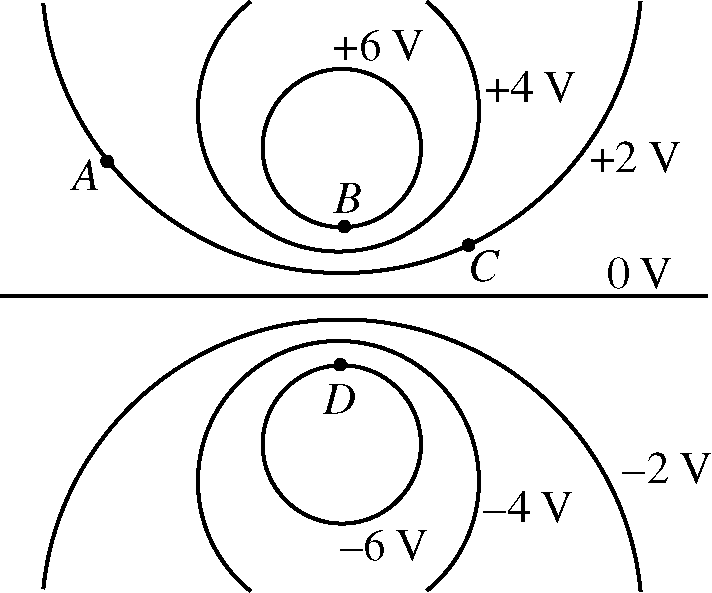
\includegraphics[scale=0.25]{images/img-009-018.png}
\end{figure}

The diagram above shows a cross section of equipotential lines produced by a charge distribution. Points $A, B, C$, and $D$ lie in the plane of the page.

% Multiple Choice Question 23
\begin{questions}\setcounter{question}{22}\question
For which two points can a negatively charged particle be moved from rest at one point to rest at the other with no work being done by the electric field?

\begin{oneparchoices}
\choice $A$ and $B$
\choice $A$ and $C$
\choice $A$ and $D$
\choice $B$ and $C$
\choice $B$ and $D$
\end{oneparchoices}\end{questions}

% Multiple Choice Question 24
\begin{questions}\setcounter{question}{23}\question
A positively charged particle is moved by an external force from rest at one point to rest at another. For which of the following motions would net positive work be required by the external force?

\begin{oneparchoices}
\choice From $A$ to $D$
\choice From $B$ to $A$
\choice From $C$ to $A$
\choice From $C$ to $D$
\choice From $D$ to $B$
\end{oneparchoices}\end{questions}

% Multiple Choice Question 25
\begin{questions}\setcounter{question}{24}\question
The electric potential shown in the diagram could be created by which of the following?

\begin{choices}
\choice A ring of positive charge
\choice A large sheet of positive charge
\choice Two negative point charges
\choice Two long lines of charge: one positive and one negative
\choice A long line of positive charge and a negative point charge
\end{choices}\end{questions}

